\section{Contribution}

\subsection{Visualization framework}

\subsubsection{Structure}

One of the main issues that we had to be deal with at the beginning of the development process was the issue of how to integrate the visualizations into the ProB 2.0 API. A functioning jetty server was already available, so we had to integrate our JavaScript visualizations into the existing framework. We ran into problems at the beginning, because a Java servlet is a singleton object. We needed to create a way to let the servlet know for which visualization it should be calculating. In order to do this, we created a session based servlet. When the user wants to open a visualization, the servlet is contacted. The servlet then creates a servlet responsible for the visualization and a unique session id. When a visualization sends a \texttt{GET} request, it includes its session id. The session based servlet then forwards the request to the the servlet that is responsible for the data calculations.

The visualization communicates with the servlet by setting up a polling interval. It tells the state space if it needs the complete data set or just the changes since the last polling interval. The servlet then responds by sending the correct data (see Figure \ref{communication}).

\begin{center}
\begin{figure}[h!]
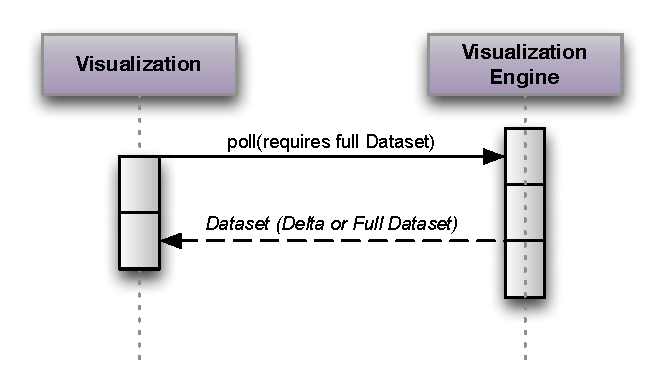
\includegraphics[width=14cm]{bilder/communication.pdf}
\caption{How visualizations communicate with the servlet that is responsible.}
\label{communication}
\end{figure}
\end{center}

The servlet is also connected to the ProB 2.0 API through the listener framework. Depending on the data that is needed for a particular visualization, the servlet registers either to receive notifications about changes in the current animation or about changes in the state space (see Figure \ref{programFlow}). Every time the servlet receives a new notification, the data needed for the visualization is recalculated.

\begin{center}
\begin{figure}[h!]
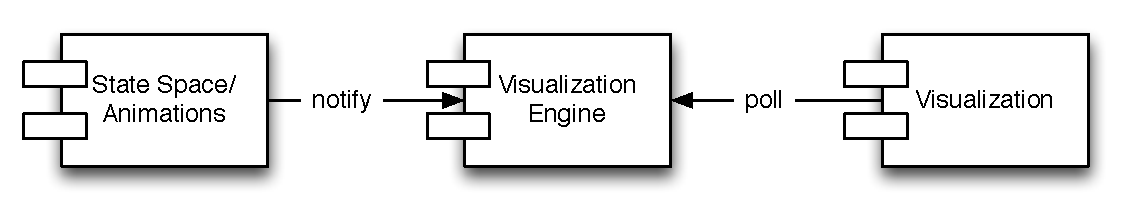
\includegraphics[width=14cm]{bilder/programFlow.pdf}
\caption{Model of the program flow.}
\label{programFlow}
\end{figure}
\end{center}

\subsubsection{User interaction with the visualizations}

Once we implemented a way to integrate the visualization servlets into the ProB 2.0 application, it was still necessary to implement an easy way for the user to interact with the visualizations. One of the main advantages of the D3 visualization framework is the flexibility for the user. Using the D3 selectors, it is possible for the user to select and change the attributes of any of the elements of the visualization. In order to offer this functionality to the users from within the ProB 2.0 application, we decided that we needed to lift the functionality from the JavaScript level into the existing groovy console in the Java 2.0 API. This was accomplished by creating a \texttt{Transformer} object that represents the action that the user wants to carry out in the visualization. Then the \texttt{Transformer} object is added to the particular visualization and is applied the next time the visualization is redrawn. The \texttt{Transformer} object was written so that its functionality is similar to what the user would actually write using the D3 library.

We wanted how the user interacted with the visualization to be as natural as possible. The user should not have a hard time learning how to manipulate the visualization. For this reason, we decided to create a small DSL that would enable the user to specify which attributes should change within a particular visualization. It is possible for the user to create \texttt{Transformers} in the console (see Listing \ref{transformer}). To do this, the user can specify a selection based on the W3C Selection API. It also specifies the attributes that should be changed for the specified selectors. The user can then apply this \texttt{Tranformer} to the servlet that is responsible for generating the data for a given transformation. To this purpose, when a new servlet is created, a variable is created in the groovy console that corresponds to the servlet in question so that the user can apply \texttt{Transformers} to the visualization directly.

\lstset{language=java}
\begin{lstlisting}[caption=Define rules for the transformation of visualization elements,label=transformer]
// Select elements with ids "rroot" and "r1" and set their fill and stroke attributes
x = transform("#rroot,#r1") {
        set "fill", "red"
        set "stroke", "gray"
}

// Apply to visualization
viz0.apply(x)
\end{lstlisting}

It is also possible to harness the power of the Groovy closure in order to create a Transformer that can be parameterized (see Listing \ref{transWclosure}).

\begin{lstlisting}[caption=Use Groovy closures to generate Transformers,label=transWclosure]
// Create a closure that can be parameterized
colorize = { selection, color ->
                transform(selection) {
                    set "fill",color
                }    
           }

// Color elements "rroot" and "r1" green
viz0.apply(colorize("#rroot,#r1","green"))
\end{lstlisting}

These \texttt{Transformers} are sent to the visualization every time that it is polled. The visualizations can then apply them. It is therefore possible for the user to manipulate the visualization. Unfortunately, in order to define these \texttt{Transformers}, the user needs to have some idea of how the elements are named internally. For the state space visualization, we also introduced an abstaction that filters a state space by predicate and produces a \texttt{Transformer} based on the states that are calculated (see Listing \ref{dynamicTransformer}). When new states are added to the state space, these will also be filtered based on the given predicate and the \texttt{Transformer} will be updated accordingly. 

\begin{lstlisting}[caption=Create a \texttt{Transformer} based on the states that match a given predicate,label=dynamicTransformer]
// Define your formula
predicate = "active\\/waiting={}" as ClassicalB

// Create a Transformer that will filter the given state space (saved in space0) according to the given predicate
x = transform(predicate, space0 ) {
		set "fill", "blue"
		set "stroke", "white"
}

// Apply the Transformer to the visualization
viz0.apply(x)
\end{lstlisting}

\subsubsection{Extensibility}

In addition to creating visualizations that are useful to the user, we also wanted to make it easy for other developers to create similar visualizations. In order to help with this, we encapsuled certain elements common to all of the visualizations into a separate script. In order to have access to these elements, a developer simply needs to include the script before that of his visualization. Currently, there are two main elements included in this script. Firstly, the user can use the \texttt{createCanvas} function to create a D3 selection that includes support for zooming (see Listing \ref{canvas}). Secondly, if the user wants to be able to apply the \texttt{Transformers} that are described in the last section, there is a built in function to apply a list of \texttt{Transformers} to the visualization (see Listing \ref{applyStyling}). In the future, it will also be possible to add more functions to this script to make it even easier to create visualizations for ProB.

\begin{lstlisting}[caption=Append a D3 selection to an element that includes support for zooming,label=canvas]
var width = 600, height = 400;
var svg = createCanvas("#elementId", width, height);

// Append all further elements to this selection
svg.append(...);
\end{lstlisting}

\begin{lstlisting}[caption=Apply list of \texttt{Transformers} received from servlet,label=applyStyling]
// The servlet has been polled, and a response has been received
var styling = response.styling

// ... Render the visualization
// ... Then apply the user defined styling
applyStyling(styling);
\end{lstlisting}


\subsection{Visualization of the State Space}

\subsubsection{Main visualization}

When a state space visualization is opened, the visualization servlet responsible for the state space visualization takes the state space associated with the current animation and extracts the information about the nodes and edges contained within the graph. This information is then processed by D3 using the force layout and rendered to create a visualization (see Figure \ref{zoomedOut}). As a basis for the visualization, we used the Force Directed Graph example created by Michael Bostock (see Appendix \ref{appendix:force}). 

\begin{center}
\begin{figure}[h!]
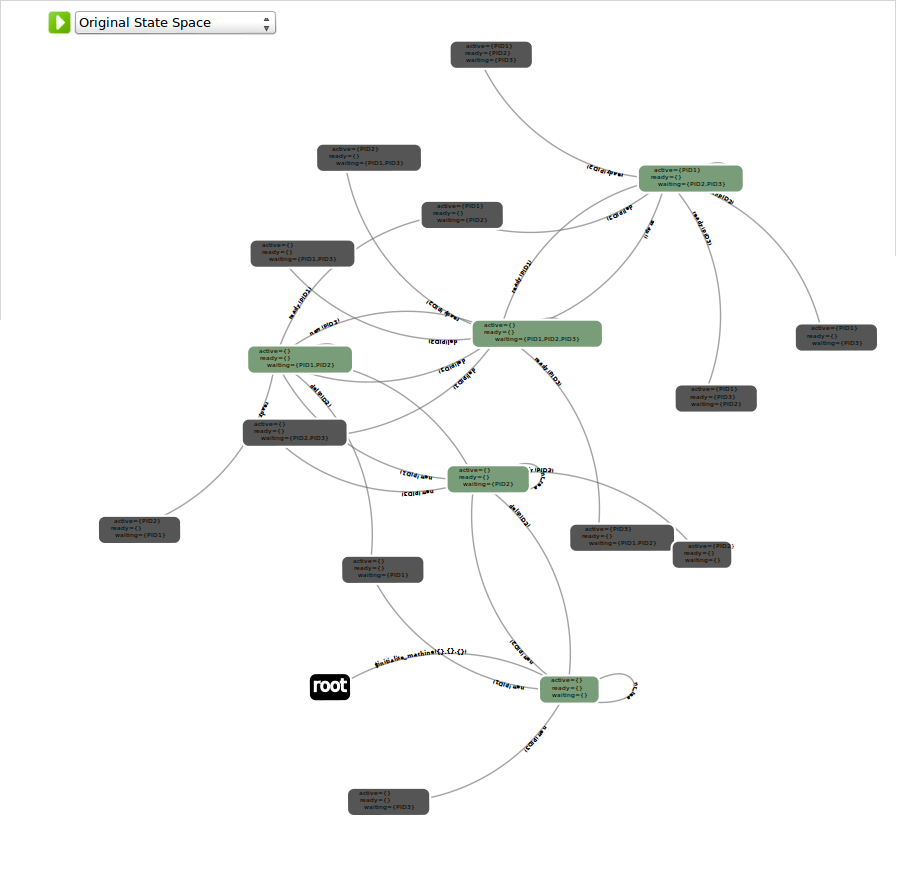
\includegraphics[width=13cm]{bilder/ss-zoomedOut.png}
\caption{Visualization of the state space for the Scheduler example}
\label{zoomedOut}
\end{figure}
\end{center}

Unfortunately, the state space contains an extremely large amount of information that has to be processed. This includes the values of the variables and the invariant for every state in the graph and the names and parameters of the operations that correspond to every edge in the graph. Because of this, it is rather difficult to create a useful visualization of the whole state space because the user not only wants to inspect how the state space appears as a whole but also the individual states within the operation. As a proposed solution of this problem, we used the zoom functionality that is available in D3. The main problem was that if the visualization of the nodes was large enough for the user to read the values of the variable at the given state, it would no longer be possible to see the state space as a whole. Instead of trying to meet both requirements at once, we simply made the text that is printed on the node and edge objects very small. When the visualization is created, the user can inspect the graph as a whole how the graph appears as a whole. The text for the given nodes, however, is virtually indiscernable. If the user wants to inspect a particular node, they can do so by zooming into the visualization. The text is then larger, and the user can see the nodes that are in the direct neighborhood of the node in question (see Figure \ref{neighborhood}). Then user can also click on the background of the visualization in order to pan through the visualization and inspect other nodes and edges. The visualization is also interactive. The user can grab a node and move it around to a desired position.

\begin{center}
\begin{figure}[h!]
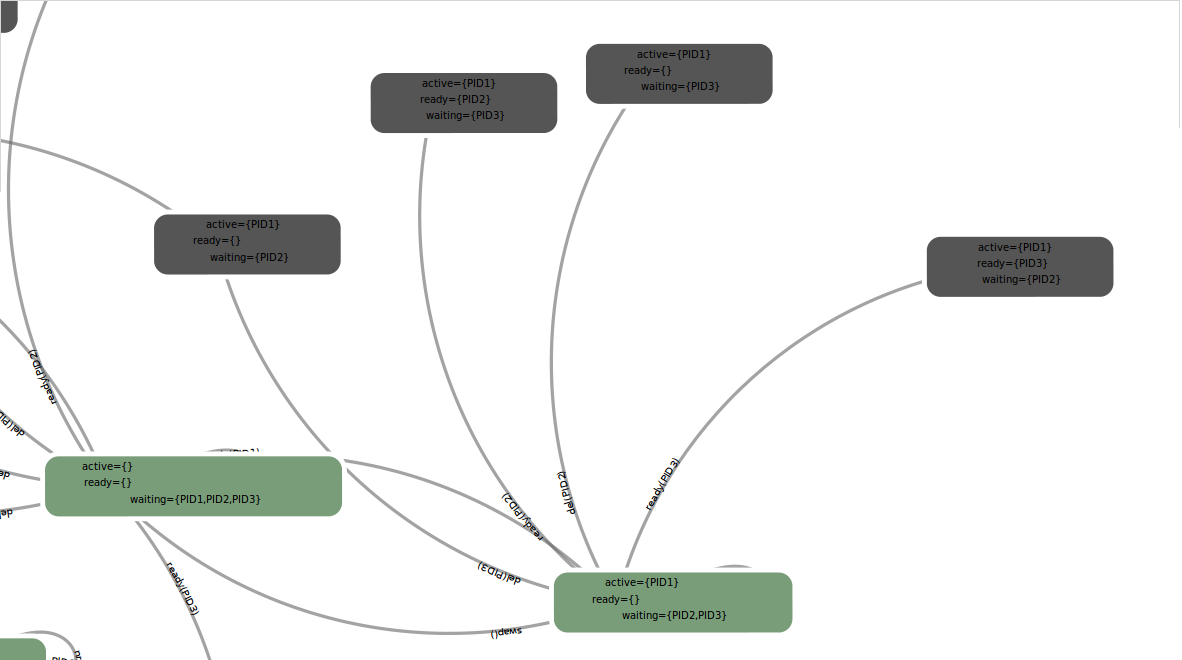
\includegraphics[width=14cm]{bilder/ss-neighborhood.png}
\caption{By zooming in, the user can inspect the neighborhood of a given state.}
\label{neighborhood}
\end{figure}
\end{center}

We had some performance issues that were associated with very large state spaces. The force layout keeps adjusting the graph until it reaches a fix point. The problem was that as the state space grew, there were more and more objects that had to be accounted for. The force layout just kept calculating and moving the the nodes. This didn't only affect the appearance of the visualization. It cost enough resources that the whole eclipse plugin would become unresponsive. A quick fix to this problem was adding a play/pause button to the upper left hand corner of the visualization (see Figure \ref{userSelect}). When the user is satisfied with the visualization and how it is laid out, he can press the pause button, and the graph will stop being rendered. When he presses the play button, the rendering will begin again. The iterative force layout keeps running in the background, so when the rendering begins again, the visualization has had time to stabilize.

When new states are added to the state space, these states are added to the graph when the visualization receives them in the next poll. The graph is then updated. This results in a nice animation.

Status about the invariant is a available in the graph based on the color of the nodes. If an invariant violation is present, the node is colored red. If the invariant is ok, the node is colored green. Otherwise, if the invariant has not yet been calculated for the given node, the node is colored gray.

\subsubsection{Visualization of Derived Graphs}

There is also support for the visualization of graphs that are derived from the state space. The ProB CLI support the generation of smaller graphs that are derived from the state space in question. These graphs show information about state space that is not obvious when dealing with the state space as whole. Two algorithms for derived graph generation are currently supported. The signature merge algorithm is supported (see Figure \ref{sigmerge}). The user can also create a transition diagram based on a user defined expression (see Figure \ref{transdiag}). 

\begin{center}
\begin{figure}[h!]
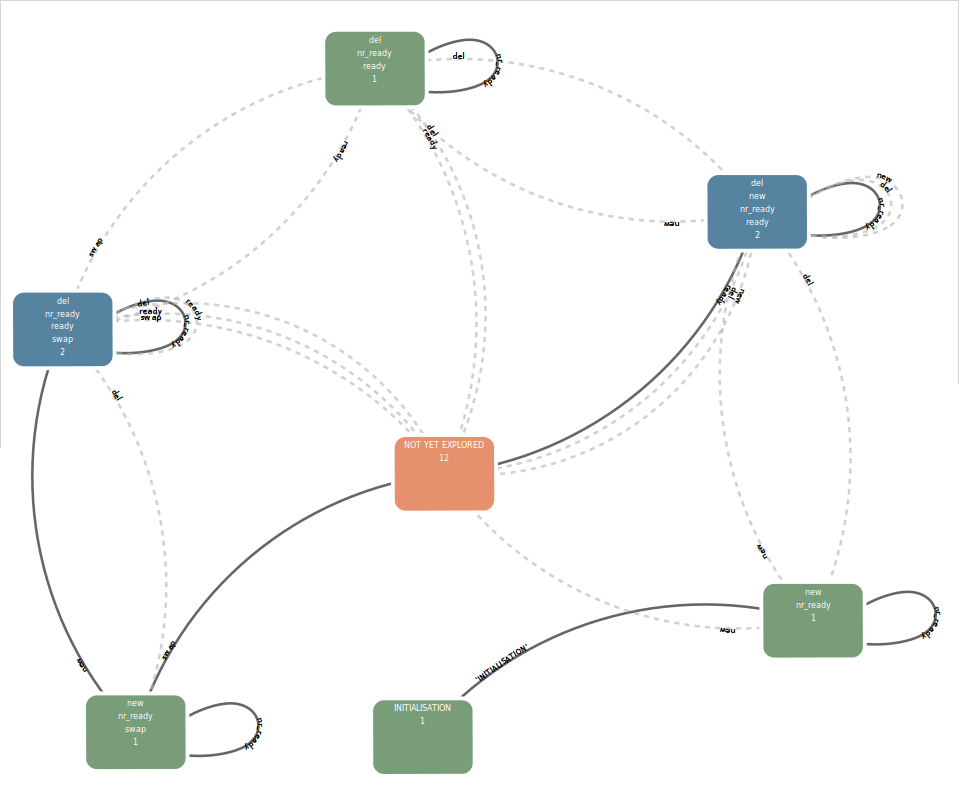
\includegraphics[width=14cm]{bilder/sigmerge.png}
\caption{D3 Visualization of signature merge for Scheduler example}
\label{sigmerge}
\end{figure}
\end{center}

\begin{center}
\begin{figure}[h!]
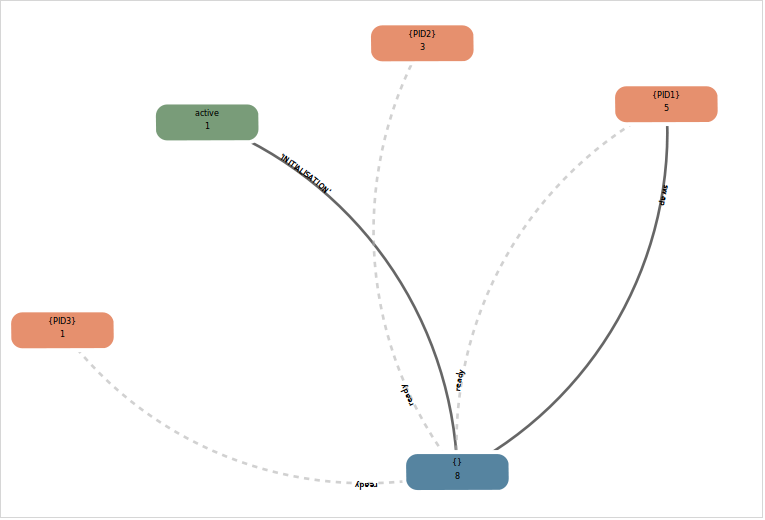
\includegraphics[width=14cm]{bilder/transdiag-wo.png}
\caption{D3 Visualization of the transition diagram of \texttt{active} in Scheduler example}
\label{transdiag}
\end{figure}
\end{center}

If the user wants to use the GraphViz algorithms and rendering engine, there is also support for both the signature merge (see Figure \ref{sigmergeDotty}) and transition diagram (see Figure \ref{transdiagDotty}).

\begin{center}
\begin{figure}[h!]
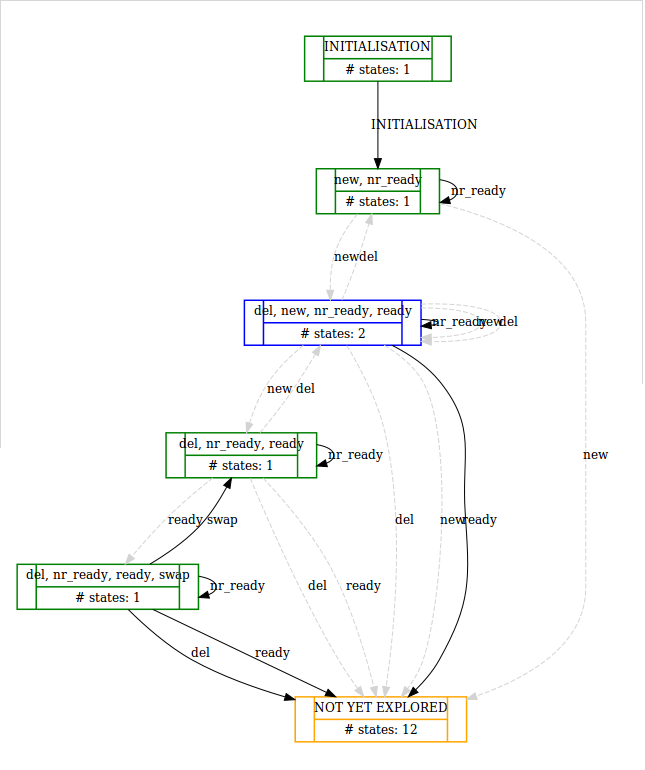
\includegraphics[width=14cm]{bilder/dotty-sigmerge.png}
\caption{GraphViz powered Visualization of signature merge for the Scheduler example}
\label{sigmergeDotty}
\end{figure}
\end{center}

\begin{center}
\begin{figure}[h!]
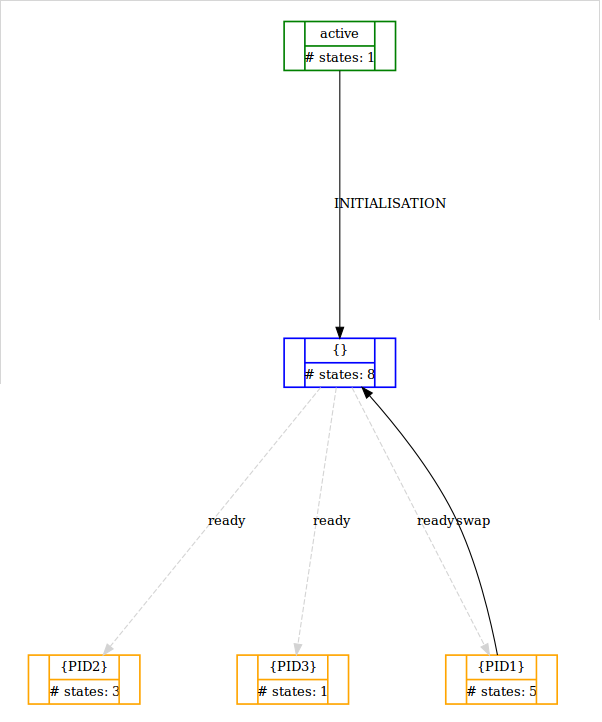
\includegraphics[width=14cm]{bilder/transdiag-dotty-wo.png}
\caption{GraphViz powered Visualization of the transition diagram of \texttt{active} in Scheduler model}
\label{transdiagDotty}
\end{figure}
\end{center}

\subsubsection{User Interface} 
There is also a basic user interface for the user to interact with the state space visualization. There is a drop down menu from which the user can decide which visualization he wants to view (see Figure \ref{userSelect}). 

\begin{center}
\begin{figure}[h!]
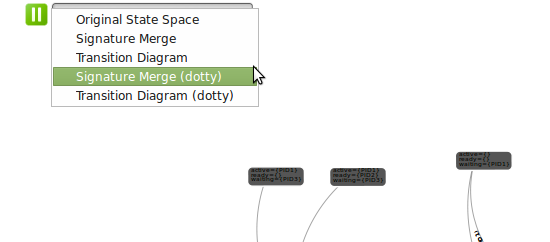
\includegraphics[width=14cm]{bilder/selectVisualization.png}
\caption{The user can select the desired visualization and play and pause the rendering.}
\label{userSelect}
\end{figure}
\end{center}

The signature merge algorithm is calculated based on the events in the model that is being animated. By default, all events are selected, but it is also possible for a user to disable events when calculating the signature merge algorithm. In the state space visualization, if the user is dealing with the signature merge graphs, a settings icon appears and the user can click on it and select or deselect the events that are of interest to him (see Figure \ref{sigMergeUI}).  

\begin{center}
\begin{figure}[h!]
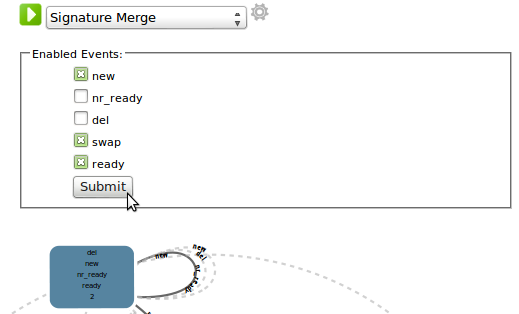
\includegraphics[width=14cm]{bilder/sigMergeUI.png}
\caption{User interface to chose events for signature merge.}
\label{sigMergeUI}
\end{figure}
\end{center}

When the user chooses to create a transition diagram from the menu, a prompt appears and the user can input the desired transition. When the transition diagram is calculated, a text field appears. In order to change the expression for a given transition diagram, the user can type it in the text field and submit it (see Figure \ref{transDiagUI}). The algorithm will then be recalculated and the graph will be rerendered.

\begin{center}
\begin{figure}[h!]
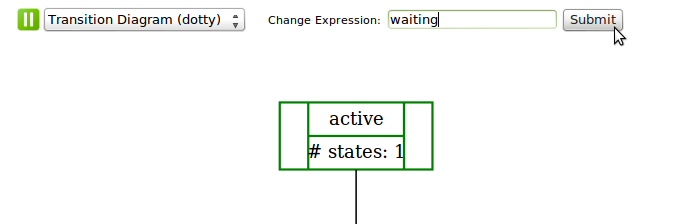
\includegraphics[width=14cm]{bilder/transDiag-UI.png}
\caption{The user can input a new expression to recalculate the transition diagram.}
\label{transDiagUI}
\end{figure}
\end{center}

\subsection{Visualization of a B-type Formula}

The ProB CLI already supported the functionality of expanding a formula into its subformulas and finding its value at a given state. However, the expanding of the formula took place lazily. A formula would be sent to the ProB CLI and then the direct subformulas of this formula would be sent back. The software would then have to contact ProB CLI recursively until all of the subformulas had been calculated and cached on the Java side. For the predicate visualization, we wanted the formula to be completely expanded and then sent in its entirety to the ProB 2.0 API. In order to do this, we implemented a prolog predicate within the ProB CLI that performs the recursive expanding of a B formula before it is sent back to the Java API. The predicate also delivers the value of each subformula for the given state. This ensures that performance will not an issue. 

The final visualization is interactive (see Figure \ref{predicate}). If a formula has subformulas, the user can select it from within the visualization to expand or to retract the subformulas. The subformulas are always either predicates or expressions. If they are expressions, they are colored white or light grey depending on whether they have subformulas or not. If the formula is a predicate that has evaluated to true for the given formula, the node is colored green. If the formula is a predicated that has evaluated to false, node is colored in red. The value of the given formula is also printed beneath the formula. This allows the user to visually identify the parts of the formulas and their given values. 

\begin{center}
\begin{figure}[h!]
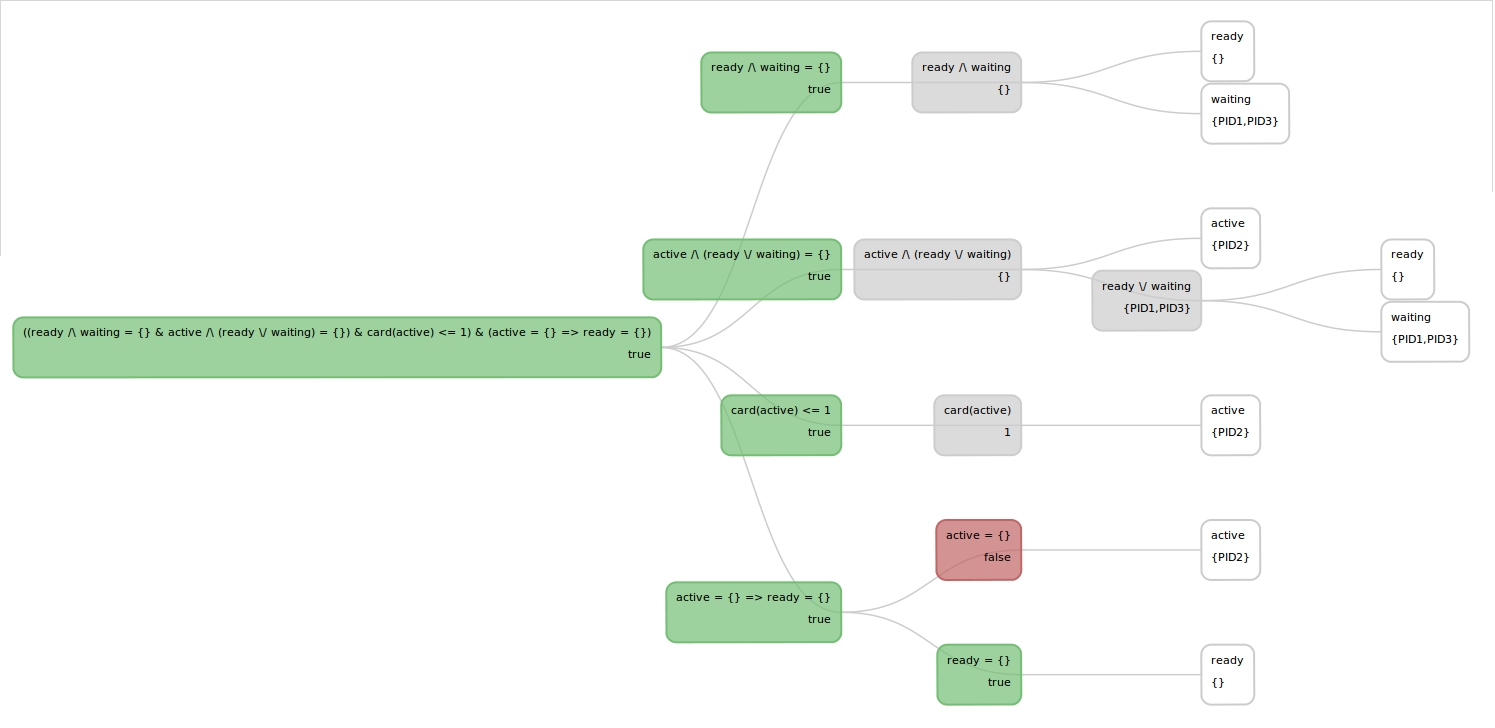
\includegraphics[width=14cm]{bilder/invariant.png}
\caption{Visualization of the invariant of the Scheduler model}
\label{predicate}
\end{figure}
\end{center}

In the implementation of the formula, the D3 tree layout is used. The expanding and collapsing of the nodes takes place with a simple JavaScript function. This visualization is based on the Collapsible Tree Layout from the D3 website (see Appendix \ref{appendix:tree}). By harnessing the power of the D3 zoom behavior, it is also possible to zoom in and out of the visualization and to pan the image to inspect it closer. The servlet responsible for the visualization implements a listener to identify if any changes in the animation occur. If they do, the formula is recalculated for the new current state, and the visualization is redrawn.

\subsection{Visualization of the Value of a Formula Over Time}

The ProB 2.0 API supports the evaluation of a given formula over the course of the history of an animation.
Because a state is defined by the values that the variables take on when dealing with B type specification languages, it can be particularly interesting to be able to examine the value of a variable over the course of a trace when dealing with a Classical B or Event-B formula. 

In order for the ProB 2.0 API to evaluate a formula, it extracts the list of states that the animation visits over the course of its history. Then it contacts the ProB CLI and extracts the value that the formlua takes on for each state in the list. This information is then processed by D3 to produce a simple line plot (see Figure \ref{timeVsValue}). As of now, formulas can only be visualized if they take on integer values. In the future, we plan to support the visualization of formulas that take on boolean values. The visualization also interacts with the ProB 2.0 API. If the current state changes, the formula is recalculated and a new plot is produced.

\begin{center}
\begin{figure}[h!]
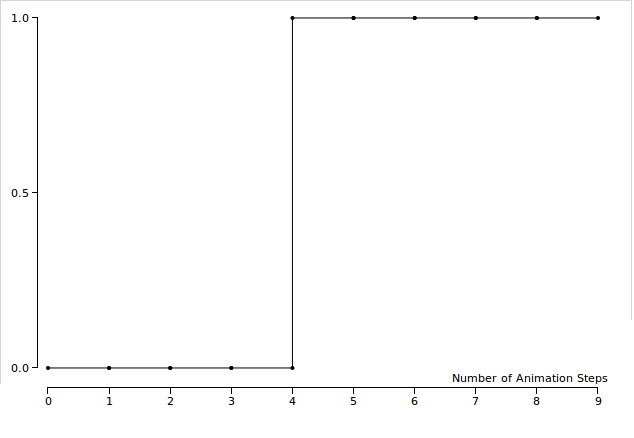
\includegraphics[width=14cm]{bilder/timeVsValue.png}
\caption{Visualization of value of \emph{card(active)} from the Scheduler model over the course of an animation.}
\label{timeVsValue}
\end{figure}
\end{center}

